

\section{The warmest and coldest day of each year}
In this work measured temperature data between 1961-2015 years for Lund have been gotten as input data then coldest and warmest days in each year are extracted and plotted by Root as the output of project in this section. It is illustrated that how appearance of coldest and warmest days are changed during the 1961-2015 period.

\subsection{Code structure}
In the 1st step, Bash scripting is performed in order to extract practical data from available "smhi-opendata-Lund.csv" file. Bash output provides required data in separate .txt files as: year.txt, month.txt, day.txt, time.txt and temperature-01.txt, this separate data file extraction strategy is for possible error checking. Only G data have been extracted and Y data considered as low quality data. In the 2nd step C++ coding is performed to process imported data in order to extract coldest and warmest days of each year. These data will tell us variation in appearance of coldest and warmest days in different years. C++ section outputs are stored in two .txt files as "WarmestDaysHist.txt" and "ColdestDaysHist.txt". In 3rd step provided .txt files from C++ are used to fill histograms, fitting histograms provide mean values as expected day for happening of coldest or warmest day in the year based on available statistics.  

\subsection{Results}
Figure 1 shows plotted results in Root for Variation of coldest and warmest days in different years between 1961-2015. Black lines show Gaussian fit, for warmest days it lead to mean value=196.5 which it is the predicted warmest day during a year in Lund. 
Following bulleted issues which are requested to be covered by performing this project are done except the fitting part related to Coldest days and getting mean value for Coldest days.

\begin{itemize}
\item   Create histograms of the warmest and coldest day each year.
\item   Predict when the warmest and coldest day is most likely to occur.
\item	Can you show both histograms in the same plot?
\item	Can you make a t function that wraps around as in Figure 3?
\end{itemize}

\begin{figure}
    \centering
    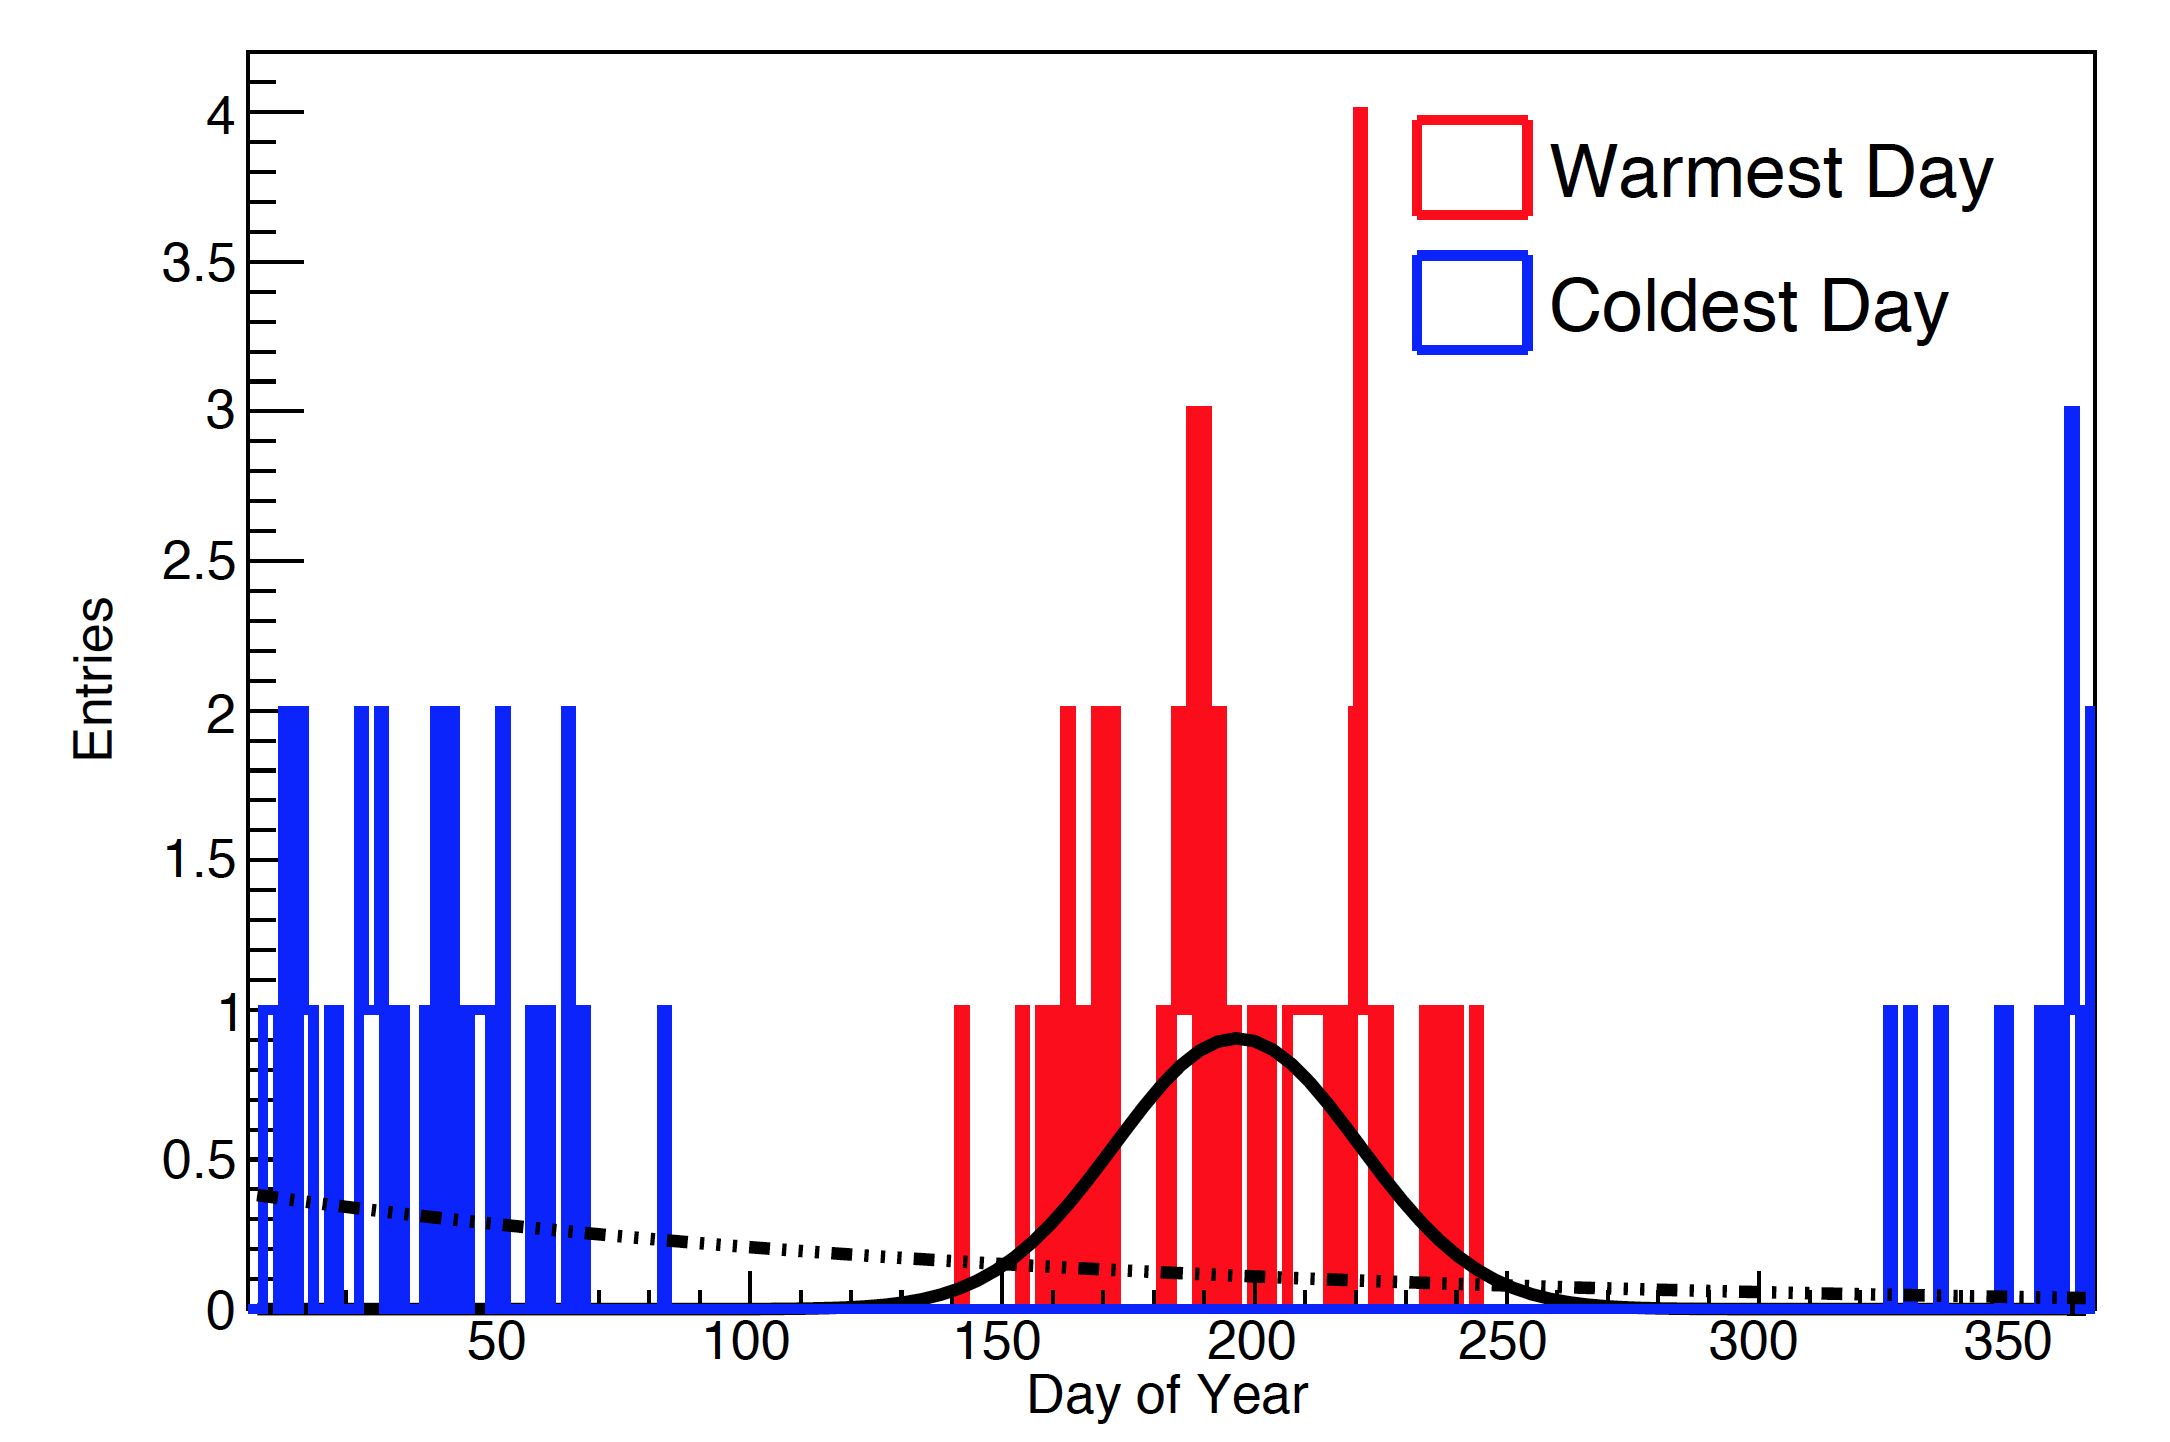
\includegraphics{0001.png}
    \caption{Variation of coldest and warmest days of year between 1961-2015. Black lines shows Gaussian fit}
\end{figure}
